\chapter{Fundamental Concepts}
\label{cap:conceitos}

This chapter presents the main base concepts used in the development of this work. Section \ref{sec:cidadesInteligentes} presents definitions and dimensions of Smart Cities and possible simulation scenarios. Section \ref{sec:simulacaoTransito} describes the fundamentals of traffic simulation, highlighting the types of traffic simulations and examples of Smart Cities scenarios already simulated. Section \ref{sec:modeloAtores} presents the actor model and the Erlang language which we used in the implementation of the InterSCSimulator. Finally, Section \ref{sec:rev_conclusoes} concludes this chapter, relating the presented concepts and the research presented in this thesis.

\section{Smart Cities}
\label{sec:cidadesInteligentes}

Most of the Smart Cities definitions highlights the expected impacts of innovative services and applications in the city population and the environment such as citizens empowerment, better quality of life, and sustainability. Other, focus on the idea of using ICT tools to create and improve the cities infrastructure and services. Table \ref{tab:definicoes} presents Smart Cities definitions that we found in the literature. Most of these definitions cite that the primary objective of a Smart City is improving the citizen quality of life. Some definitions \cite{giffinger2007smart,guan2012smart} do not establish the mean to achieve this objective, while others define that this objective will be achieved using a technological infrastructure to improve the infrastructure and services of the city \cite{caragliu2011smart,dameri2013searching,harrison2010foundations}.

\begin{table}
\centering
\caption{Smart Cities definitions found in the literature}
\label{tab:definicoes}
\smallskip
\begin{tabular}{c|c}
\hline

Definition 
& Author \\\hline

“A Smart City is a city well performing built on the\\
‘smart’ combination of endowments and activities of\\ 
self-decisive, independent and aware citizens” &  \cite{giffinger2007smart} \\\hline

“A city to be smart when investments in human and social\\
capital and traditional (transport) and modern (ICT)\\
communication infrastructure fuel sustainable economic\\ 
growth and a high quality of life, with a wise management\\
of natural resources, through participatory governance”
& \cite{caragliu2011smart}  \\\hline

“A smart city is a well-defined geographical area, in which\\
high technologies such as ICT, logistic, energy production,\\ 
and so on, cooperate to create benefits for citizens in terms\\
of well-being, inclusion and participation, environmental\\
quality, intelligent development; it is governed by a\\ 
well-defined pool of subjects, able to state the rules and\\ 
policy for the city government and development” 
& \cite{dameri2013searching}  \\\hline

“A city that monitors and integrates conditions of \\
all of its critical infrastructures, including roads, \\ 
bridges, tunnels, rails, subways, airports, seaports, \\ 
communications, water, power, even major buildings, \\
can better optimize its resources, plan its preventive \\
maintenance activities, and monitor security aspects \\
while maximizing services to its citizens”
& \cite{hall2000creative} \\\hline

“A city connecting the physical infrastructure, the\\
IT infrastructure, the social infrastructure, and the\\
business infrastructure to leverage the collective\\
intelligence of the city”
& \cite{harrison2010foundations} \\\hline

“A smart city, according to ICLEI, is a city that is\\ 
prepared to provide conditions for a healthy and happy\\
community under the challenging conditions that global,\\
environmental, economic and social trends may bring.”  & \cite{guan2012smart} \\\hline

“The use of Smart Computing technologies to make the\\ 
critical infrastructure components and services of city\\
which include city administration, education, health-care,\\ 
public safety, real estate, transportation, and utilities\\
more intelligent, interconnected, and efficient”
& \cite{washburn2009helping} \\\hline

\end{tabular}
\end{table}

Most of the Smart Cities definitions cite the necessity of using Information and Communication Technologies (ICT) to improve the use of the city infrastructure, the resources management, and the city services \cite{harrison2010foundations,washburn2009helping}. Some definitions also cite the importance of sustainability in the city, making more efficient use of resources such as water and electricity \cite{caragliu2011smart,dameri2013searching}.

Another important discussion is the necessity of leveraging the economic development of the cities \cite{dameri2013searching}, facilitating the integration and participation of the whole city population. Two definitions \cite{dameri2013searching,giffinger2007smart} cite the importance of participatory governments allowing the citizens define the cities priorities.

Also regarding ICT, some definitions cite that Smart Cities applications and services should monitor the cities infrastructure such as streets, bridges, train lines and stations, and public buildings \cite{hall2000creative}. Also, they must monitor and control their resources such as water and electricity \cite{hall2000creative}. Finally, the data collected in the city monitoring must be available and integrated to facilitate the creation of Smart Cities applications and services \cite{harrison2010foundations,washburn2009helping}.

Besides the Smart Cities definitions, Giffinger et al. \cite{giffinger2007smart} describe six dimensions to measure the smartness of a city. The dimensions are: \textit{Smart Economy}, \textit{Smart People}, \textit{Smart Governance}, \textit{Smart Mobility}, \textit{Smart Environment} and \textit{Smart Living}. Many authors already use this classification \cite{munoz2011forefront,papa2013towards} and there is a benchmark used to rank the smartest cities in Europe using these dimensions.\footnote{Smarts Cities in Europe - \url{www.smart-cities.eu}} The definition of each dimension is in the following:

\begin{itemize}

    \item \textbf{Smart Economy} measure the economic development of the city through parameters such as the quality of the enterprises in the city and the city entrepreneurship ecosystem. Examples of initiatives related to this dimension are incentives to companies for the development of technological solutions for the city and the improvement of the business environment with adequate legislation and business infrastructure. 
    
    \item \textbf{Smart People} is related to the development of the city's population using parameters such as education, employment rate, and income. Some actions related to this dimension are projects for digital inclusion of citizens and programs for scientific and technological education. 
     
    \item \textbf{Smart Governance} access the quality and transparency of municipal public agencies with parameters such as ease of use of public services, investments in technology, and transparency in the public data and the use of city resources. Some actions related to this dimension are the creation of participatory governments and the dissemination of information about the city in transparency and open data portals.
 
    \item \textbf{Smart Mobility} measures the ease of mobility in the city in the various modes of transportation such as bus, subway, car, and bicycle. It uses parameters such as kilometers of congestion, subway network size and the number of people using public or non-polluting transportation. Some actions related to this dimension are real-time monitoring of streets flow, the use of sensors to indicate free parking spots and applications to facilitate and encourage the use of public and sustainable transport, such as bicycles and electric vehicles.
 
    \item \textbf{Smart Environment} check the sustainability of the city using parameters such as environmental pollution, efficiency in the use of city resources such as water and electricity, and the amount of recycled waste. Some actions related to this dimension are the measurement of the city's air and water quality, the use of renewable energy sources and the real-time measurement of the resources used in buildings.
    
    \item \textbf{Smart Living} evaluates the quality of life of the population using parameters such as entertainment, security, and culture. For example, counting the number of green areas, the number of libraries and homicide rate of the city. Some actions related to this dimension are the use of elderly health monitoring applications, automatic image processing of security cameras and applications that show the cultural events programmed in the city.

    
\end{itemize}

There are a plenty of Smart Cities initiatives around the world, most in Europe \cite{caragliu2011smart,manville2014mapping}, several in the United States \footnote{10 Smartest Cities in USA - \url{www.fastcoexist.com/3021592/the-10-smartest-cities-in-north-america}}, Japan and China \cite{liu2013smart} and some other project in other countries such as Brazil \cite{fortes2014deployment}, United Arab Emirates \cite{janajreh2013wind} and South Korea \cite{kshetri2014development}. These data show that the vast majority of projects are concentrated in developed countries, there are a few projects in developing countries. In Brazil, there are already several initiatives such as in S\~ao Paulo, B\'uzios, Recife, and Joinville. We did not find any project in the poorest countries of the globe. Figure \ref{figure:mapa} shows a map of the initiatives found in the literature or pages of the projects.

\begin{figure}[!htb]
\centering
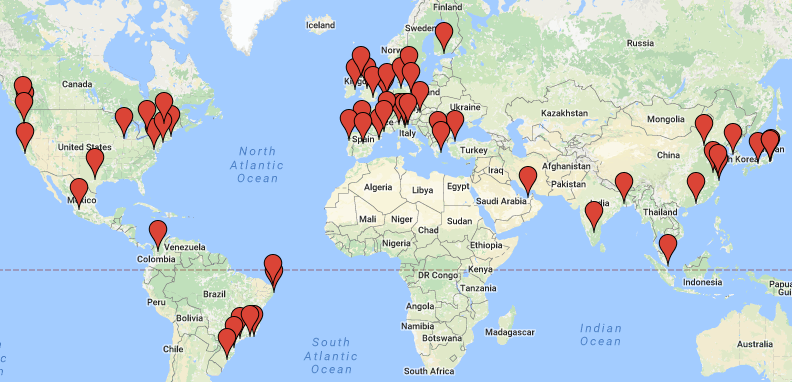
\includegraphics[height=7cm]{figuras/mapaCidades}
\caption{Smart Cities initiatives around the world}
\label{figure:mapa}
\end{figure}

Some examples of very advanced initiatives in Smart Cities are Santander, Spain, which through the SmartSantander project has already deployed an extensive sensor network in the city to collect data such as temperature, vacant parking spot and noise levels in the city streets. Amsterdam, which has a variety of Smart Cities projects such as encouraging the use of electric cars, bicycles and public transport, automatic monitoring of the city conditions and the use of a smart electricity distribution network. Barcelona, Spain, which has several projects to increase citizens' participation in city decision-making and to make data available on public administration openly.

The next sections present Smart Cities initiatives, applications, and services already implemented in cities around the world. Based on these initiatives, we derived possible scenarios that are possible to simulate in a Smart City simulator.

\subsection{Smart Economy}

This subsection presents projects related to the economic growth of the city, attracting investments and creating more and better jobs. Examples of services and applications of this field are associated with tourism, efficient usage of city resources and the attraction of enterprises and startups to the city. 

In Santander, researchers developed an augmented reality application to smartphones which contain plenty of information of more than 2700 points of interest in the city such as museums, bookstores, buses stop, tourism office, and bicycle rental stations. The application also shows the position of buses and taxis in real-time \cite{sanchez2014smartsantander}. Figure \ref{figure:santanderRa} presents the main screen of the applications, which shows the information of a bus line and a point of interest of the city.

\begin{figure}[!htb]
\centering
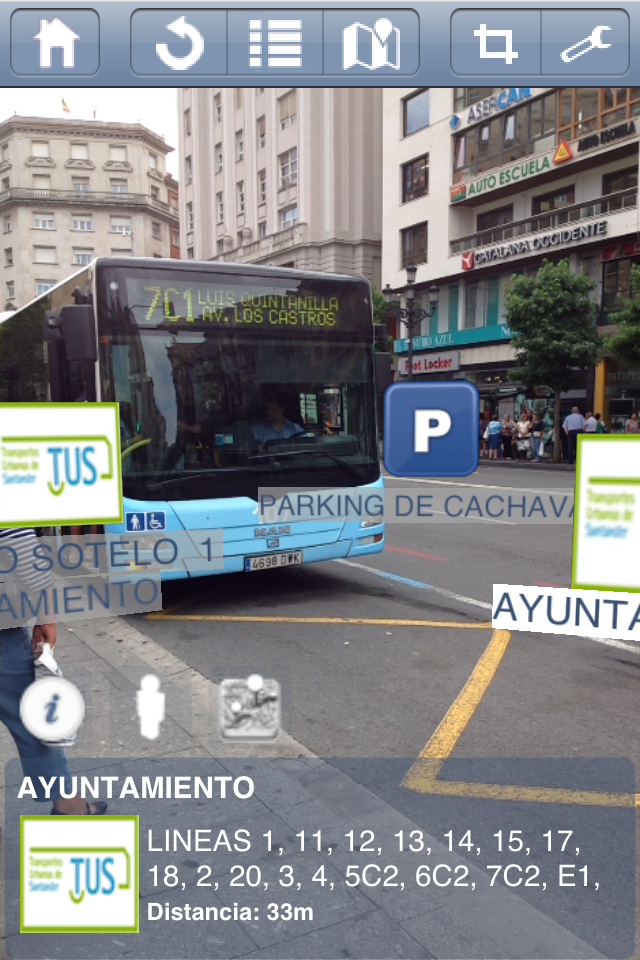
\includegraphics[height=10cm]{figuras/santanderRA}
\caption{SmartSantander augmented reality application}
\label{figure:santanderRa}
\end{figure}

In Cagliari, Italy, the municipal government has developed a platform based on the Internet of Things and Cloud Computing to collect data and create services for tourists in the city \cite{nitti2017iot}. To test the platform, they developed a case study in which a tourist selects a list of Points of Interest (POIs) that they want to visit in the city. Each PdI has a variety of static data, such as address and hours of operation, and data captured in real time, such as the size of the entrance queue and the current number of visitors. With this data, the application calculates the best sequence of PdIs that the tourist should visit. The purpose of the application is to optimize the time of the tourist, allowing him to be able to visit as many attractions as possible in the time that he is in the city.

Also related to tourism in Amsterdam, the government has adopted the CitySDK Tourism API \cite{pereira2015citysdk}, a tool that allows the development of applications to help tourists visiting the city. This tool collects data from the city's open data portal, which is in CSV, XLS, and text files and makes them available in an easy-to-access and processing API for third-party applications. Some of the shared data are city landmarks such as museums, parks and historic buildings, events that are happening in the city and tourist itineraries.


Búzios is one of the first cities in Brazil to start a project for the implementation of a Smart City infrastructure \cite{fortes2014deployment}. The main purpose of the project is to make the city more sustainable, using resources rationally and efficiently. Among the main actions carried out in the city is the implantation of an intelligent electric energy network, the creation of intelligent buildings and the improvement of the communication systems of the city using technologies such as Wi-Fi, Mesh networks, and Power Lines Communication (PLC).

Also in Amsterdam, the government deployed the first Smart Electricity Grid in a region of the city with approximately 10,000 houses. In this network, it is possible for c to consume and produce energy and to monitor energy usage in their homes in real time. Also, this project also facilitates the monitoring and maintenance of the network by city authorities.

In this application domain, researchers can develop simulations of a Smart Grid, comparing the cost and the emission of pollutants in the use of diverse sources of electrical energy and simulating the network of distribution, production, and consumption of energy. They can also simulate buildings that attract large numbers of people, such as sights and places of big events, making it possible to understand their impacts on the city's traffic.

\subsection{Smart Population}

This subsection presents projects aimed at improving social parameters related to the population of the city such as education, employment, and income. Moreover, some researchers discuss the empowerment of citizens with data that allow them to make better political choices. Examples of services and applications in this area are related to education such as initiatives and applications for improving education and facilitating the digital inclusion of city citizens and improving the city's business environment by increasing the quantity and quality of jobs.

An initiative in England teaches students to work with data sets related to the city \cite {wolff2015education}. The idea is to enable citizens to know the tools to analyze the data independently of the will of companies or city rulers. The purpose of this work is to extend class activities with activities such as Hackathons aimed at the development of applications and services for the city. The researchers already did tests using datasets on the use of electricity in the city.

In Barcelona, the municipality created a laboratory (Barcelona Urban Innovation Lab Dev), which investigates various urban problems and fosters the participation of the private sector in the development of products and services related to the improvement of urban space \cite {bakici2013smart}. The laboratory provides human resources and tools to support the development of these solutions. The objective of this laboratory is to attract companies to develop tools for the city, creating jobs that need high qualification and also creating solutions to improve quality of life in the city.

Scenarios linked to education can be simulated in this area such as schools and universities, and from which part of the city these institutions attract the population. So governors and private schools can choose the best area for the creation of new schools or university campuses and also measure the impact on the city traffic.

\subsection{Smart Governance}
\label{subsec:governanca}

This subsection presents projects related to the governance of the city. The main objectives of this type of projects are facilitating the city administration and enable the citizen participation in the city decision-making. Examples of services and applications in this field are platforms to city monitoring, open data portals, and the encouragement of the citizens to participate in the city decisions.

Seattle is considered by some rankings the smartest city in the United States \footnote{\url{https://goo.gl/5xAhh9}}.
There, researchers performed a survey \cite{alawadhi2013aspirations} with citizens and public agents asking what the main services, applications, and initiatives that the city are developing to improve the citizens' quality of life are. Among the cited projects are the open data portal \footnote{Seattle Open Data - \url{data.seattle.gov}}, the infrastructure to support the use of electric vehicles, and the use of Customer Relationship Management (CRM) to control the communication between the city government and the citizens. According to the survey, the benefits of these actions are the improvements in the city services, the reduction of the city expenses, and electrical energy saving. 

In Chicago, the municipality developed the platform WindyGrid \cite{thornton13windygrid}, which collects, stores, and process the data of the city. The objective of this platform is providing a unified platform to city operators visualize the city operation in real-time. Examples of the collected data are calls to the emergency service (911), events in the city traffic, publications about the city in social networks, and data regarding the public buildings. The WindyGrid provides three main functional requirements to the city managers: incidents monitoring though emergency calls and social networks mining, historical data visualization, and real-time analyses of events in the city.


In Amsterdam, there are many projects to leverage the city management transparency, especially the city expense and the decisions of the city government. For example, the Budget Monitoring allows citizen and NGOs access and suggest changes to the city budget and the Smart City SDK, which provides access to the real-time city data to application developers, including data about the city traffic, airports arrivals and departures, and the climate. Finally, to facilitate the participatory government, the city developed the AmstermOpent, a platform that allows the citizens to suggest actions and works in the city.

Many cities around the world already provide access to the city documents through open data portals allowing citizens to supervise the government expense and actions. For example, Barcelona\footnote{OpenData BCN - \url{opendata.bcn.cat/opendata/ca}} make available a big number of data about the city administration such as the city budget and expenses, municipal services stats, and data about the city population. Dublin, in Ireland, also has a completely open data platform called Dublinked \cite{stephenson2012open} which provide access to more than 200 datasets offering historical and real-time data. Moreover, using Web Semantic tools, it is possible to link the data from the platform automatically.

S\~ao Paulo has many open data projects such as the open data portal of the city \footnote{Dados Abertos São Paulo - \url{saopauloaberta.prefeitura.sp.gov.br}}, and GeoSampa\footnote{GeoSampa - \url{geosampa.prefeitura.sp.gov.br}} which provides different georeferenced datasets such as the location of public equipment, buses stops, and flood points in the city. Another example is the Olho Vivo API \footnote{API Olho Vivo - \url{www.sptrans.com.br/desenvolvedores/APIOlhoVivo.aspx}}, which allows the monitoring in real-time of all the buses in the city. This API allowed the development of many applications to facilitate the mobility in the city by buses such as Moovit\footnote{Moovit - https://goo.gl/FMYk8u} and Coletivo\footnote{Coletivo - https://goo.gl/QBvoNc}.

Another tool extensively used by the cities to share their data with the citizens is the dashboards. Usually, these tools present real-time data in a city map with various information about the city such as climatic conditions, air quality, traffic conditions, and state of the public equipment. One dashboard example is the Dublin dashboards\footnote{Dublin Dashboards - \url{www.dublindashboard.ie}}, which provides different data about the city such as temperature, air quality, noise levels, and level of the rivers in the city. Figure \ref{figure:mapaDublin} presents an example of the city dashboard displaying data of the city traffic.

\begin{figure}[!htb]
\centering
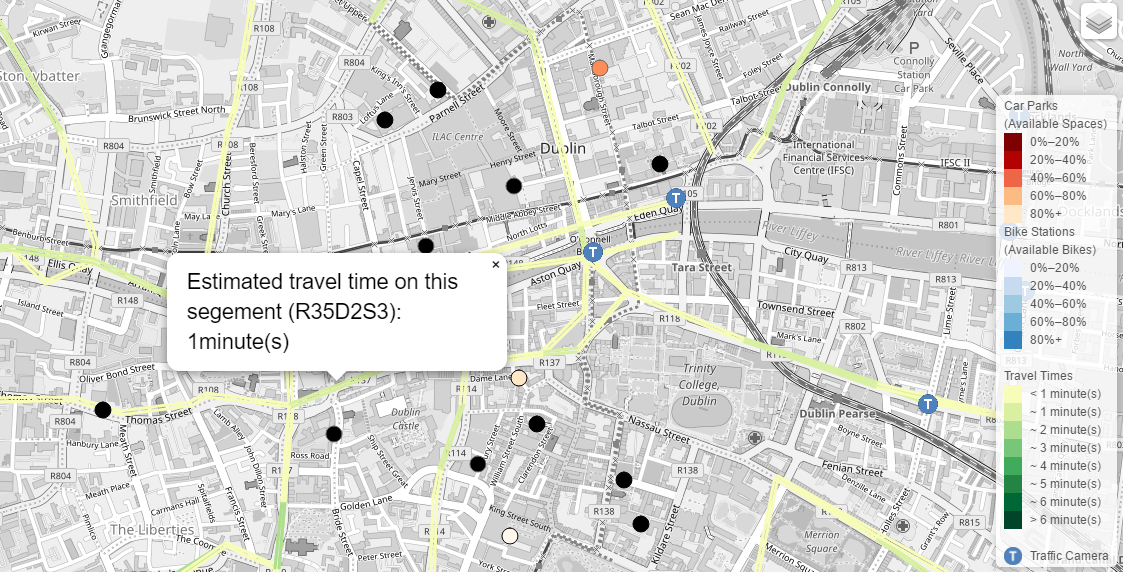
\includegraphics[scale=0.5]{figuras/mapaDublin}
\caption{Dublin Dashboard showing available park spots, available bikes in bikes stations, and the traffic situation in avenues in the city}
\label{figure:mapaDublin}
\end{figure}

This Smart City domain is linked to tools for monitoring the city, and we did not think in any scenario that can be simulated. However, a Smart City simulator can assist in tests and experiments of applications cited in this subsection, enabling the generation of workloads such as sensor and traffic simulation for the creation of monitoring applications.

\subsection{Smart Mobility}

This subsection presents projects related to mobility, which has the main objective of improving the people flow in the city and monitor the mobility infrastructure of the city such as roads and subway stations. There are plenty of examples of Smart Mobility services and applications such as traffic monitoring through security cameras, best route services, smart parking applications, and applications to show the best route using public transportation.

With the SmartSantander platform, a research project developed an infrastructure to show the free parking spots in the city. Moreover, it creates a service to predict the use of the spots during events in the city \cite{vlahogianni2014exploiting}. This service has the objective of avoiding that drivers lose time searching for a parking spot in the city, what increases the traffic in the city and the emission of polluting gases. Figure \ref{figure:smartsantandermap} presents the monitored parking spots in the city map.

\begin{figure}[!htb]
\centering
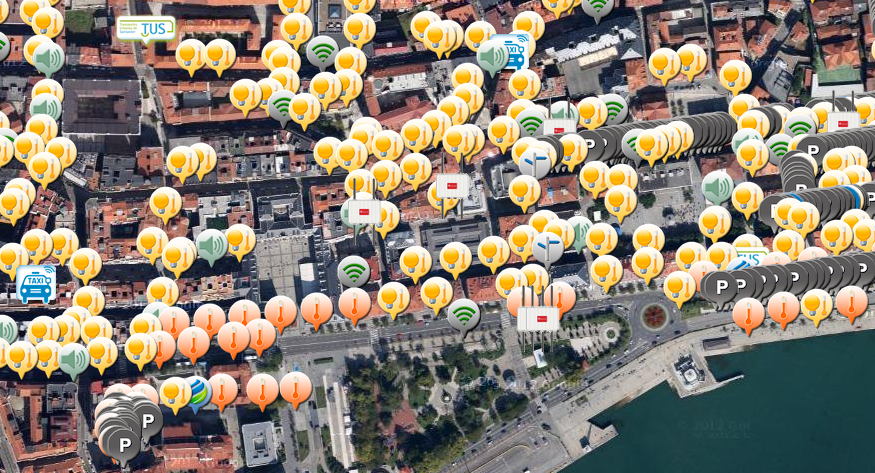
\includegraphics[height=8cm]{figuras/smartsantandermap}
\caption{Map with the monitored parking spots in the city of Santander}
\label{figure:smartsantandermap}
\end{figure}

The city of Barcelona also has a project to encourage the use of sustainable transportation modes. For example, the city developed a large infrastructure to facilitate the use of electric cars with more than 300 recharge points deployed in the city. Moreover, the city is promoting the use of shared bicycles and provided more than 400 loan stations to the citizens.

Amsterdam is also implementing several solutions in the area of traffic control and monitoring. For example, projects under development in the city are: encouraging the use of electric cars, providing battery recharging stations in various parts of the city, monitoring the main city roads for the rapid attendance of traffic problems, reservation of parking spaces in the city, avoiding the search for a vacancy, reducing the emission of $CO_2$, and the incentive to use bicycles.

In Madrid, researchers developed other two projects. The first was an application to smartphones to facilitate the commuters to find the best route using public transportation in the city. The applications also used contextual information to find best routes such as the user location and the city weather. The second application uses the user's smartphones to estimate the number of people inside a bus. People expecting for a bus can use this information to decide if it worth to take the bus or wait until the next one.

In S\~ao Paulo, the startup Scipopulis \footnote{Scipopulis - www.scipopulis.com} developed a Bus Panel used by the São Paulo Transport Secretariat (SPTrans) and the Company of Traffic Engineering (CET). This application monitors the more than 14,000 city buses and shows the speed of buses in real time on all the streets and integrates data from various sources (GPS positions of buses, segregation of the road, accidents, etc.). This information is contextualized regarding the time of day, type of road (corridor, track or shared road), accidents in the region and amount of bus passing through that route. The operator can monitor entire bus lines or sections of a line, and view the history of speeds for each street segment. The city transport network planning, operation and management teams use the panel to identify chronic bottlenecks, contingency problems, identify ways to implement buses single lanes and corridors, and the times at which the buses should operate. Figure \ref{figure:scipopulis} shows a screen of the Bus Panel application.

\begin{figure}[!htb]
\centering
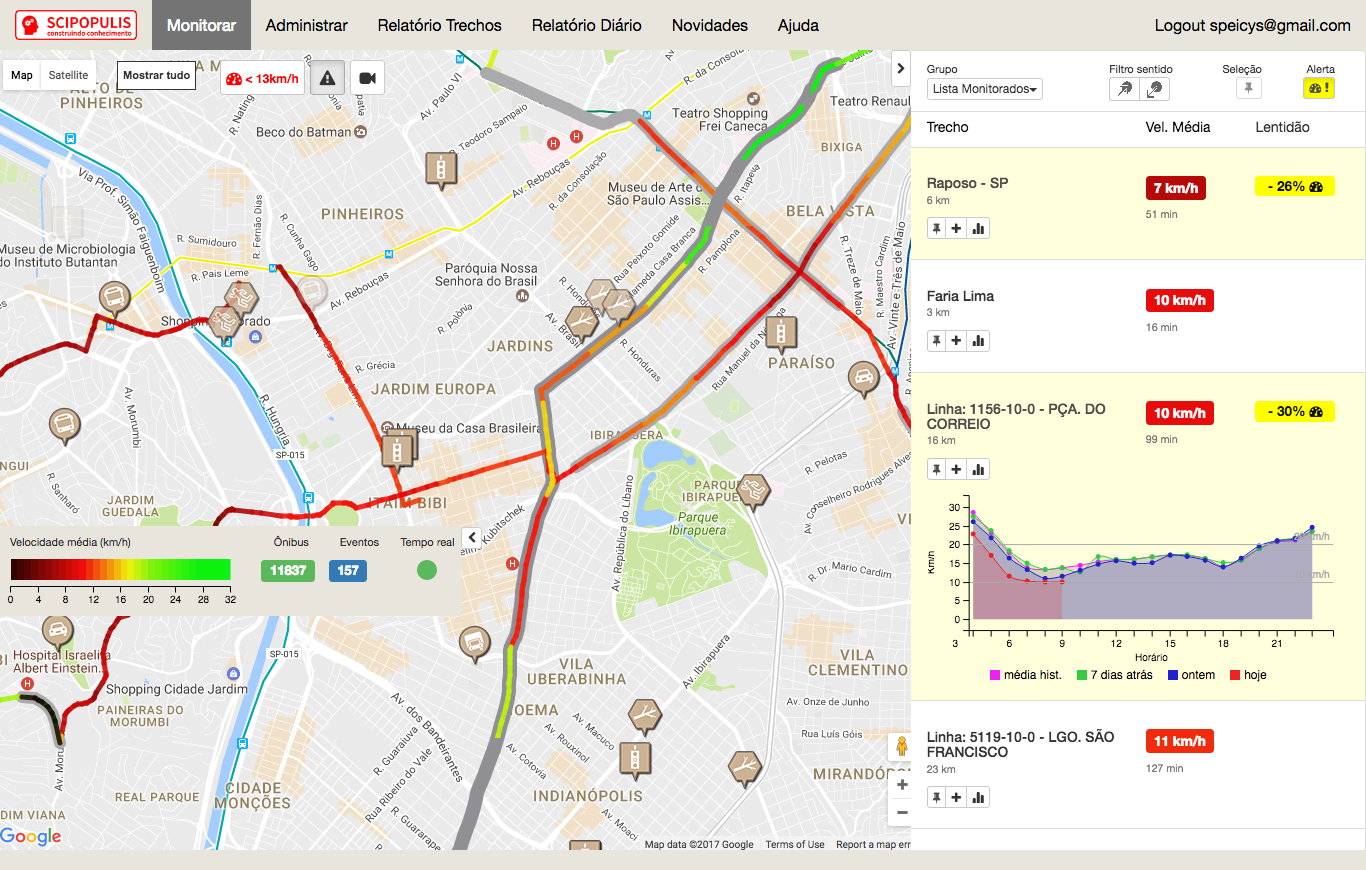
\includegraphics[scale=0.30]{figuras/scipopulis}
\caption{S\~ao Paulo bus dashboard showing the speed of the buses in the main avenues and bus corridors in the city}
\label{figure:scipopulis}
\end{figure}

In the dimension of Smart Mobility, it is possible to simulate a large number of scenarios such as the movement of vehicles in the city, compare various parameters in the road network such as increasing or decreasing street speed, accidents, and problems in roads such as floods or protests. It is also possible to simulate the public transportation of the city such as buses and subways, comparing the city traffic by increasing or decreasing the number of users on public transport, searching for the best route to a new bus line and analyzing the impact of new subway lines.

\subsection{Smart Environment}

This subsection presents projects related to the environment. Most of them have the objective of making the city more sustainable improving services such as garbage collection and recycling, efficient distribution of resources such as water and electricity, and reducing air and water pollution in the city.

Masdar is a neighborhood in the city of Abu Dhabi in the United Arab Emirates built with the objective of testing several initiatives of Smart Cities. The areas tackled in the project are the use of renewable energy sources, the conscious use of water and the reduction of the amount of garbage generated. Also, the city was planned with an intelligent transportation network to reduce the need for the use of individual vehicles, reducing the emission of pollutants. In this neighborhood, all buildings are designed in a way that saves resources and produces their energy with the use of solar panels.

In Manchester, the city is developing a project to build smart houses. In this houses, the citizen can monitor in real-time the use of resources such as electric energy and water. The objective of this project is to decrease the pollution emission and save the natural resources of the city \cite{manville2014mapping}.

The city of Santander has implemented a project to manage garbage collection in the city\cite{munoz2017santanderlixo}. This project uses data from more than 1000 sensors that monitor how full the city dumps are. Also, it is possible to monitor garbage trucks and garbage dumps. This system allows garbage trucks to visit only dumps that are full, reducing the distance that the trucks must travel. Three significant benefits of this service are the decrease in the truck expenses, the reduction of emissions of pollutants by the vehicles and the better management of the garbage collected in the city. Barcelona also has a similar project in which it is possible to monitor the current state of the garbage dumps in the city. Figure \ref{figure:sentilo} shows the city map with the sensors in the dumps.

\begin{figure}[!htb]
\centering
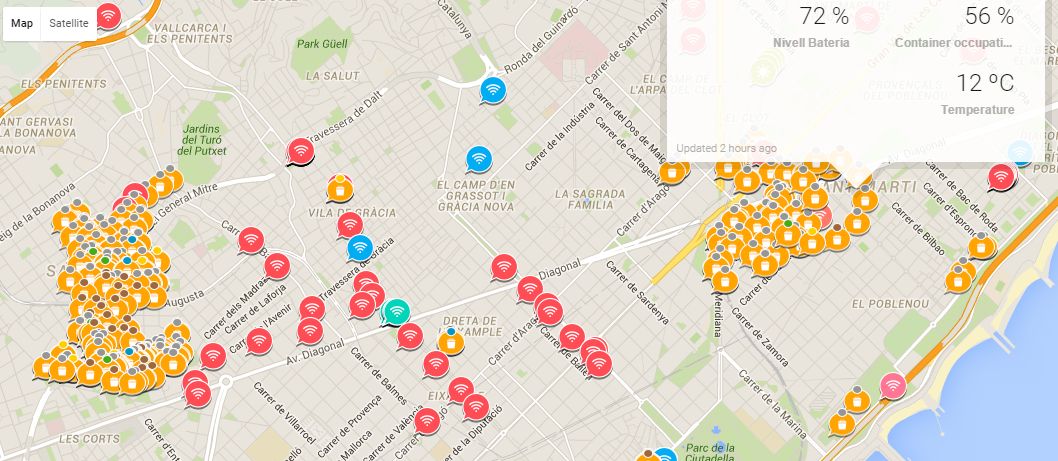
\includegraphics[scale=0.5]{figuras/sentilo}
\caption{Sensors indicating the amount of garbage in the city dumps in the Sentilo platform}
\label{figure:sentilo}
\end{figure}

Also in Santander, the city is deploying a Smart Light project, which installed more than 20.000 LED lamps with a movement detection system. This system turns on the lamp only when it detects a person is moving close from the lamppost. Also, along with the system, the smart lamps also allow the monitoring of the state of the lamp, facilitating the detection of problems in the system. With this project, the city plans to reduce 80\% the electric power consumption with the public lighting. Also, the city expects to reduce the expenses with the maintenance of the system, because currently the maintenance is made through rounds across the city.

A district of Barcelona is already operating a system for heating and cooling buildings \cite{hug2016barcelona}. The system works with a water network that passes through several district buildings, mainly public building and using the energy generated by the city's waste incinerators heat or cool the water in the pipeline. The city estimated that this system uses 35\% less power and reduces pollutant emissions by 50\% than conventional systems heating systems.

In the dimension of Smart Environment, it is possible to simulate the impact of different initiatives in the environment. For example, the emission of pollutants by the car fleet of the city, the variation in the emission if more people use public transportation, and the impact of using electric vehicles. Also, it is possible to simulate the environmental impact of the use of different electric power sources such as hydroelectric, wind, and solar. 

\subsection{Smart Living}

This subsection presents projects related to the improvement of citizens' quality of life. These project aims to improve services that are directly related to citizens' routine, such as security, cultural activities and sports activities. Examples of services in this dimension are applications that warn of events taking place in the city, for monitoring crowded areas, and for reporting problems in public places such as parks and government buildings.

In Santander, researchers installed a network of more than 20 thousand sensors and actuators in the city. This sensor network collects a vast amount of data in various regions of the city such as temperature, free parking spaces, points of interest and luminosity. The data collected is used for the development of applications and services that improve the quality of life of the citizens. Figure \ref{figure:smartsantandermap} shows a map in which each point is a device deployed in the city that sends data to the platform. An example of an application developed with the data of the sensor network is one that reminds the city population of events that will occur in the city. Besides the event, the application also sends information about the region of the event to the users such as parking spots, noise levels, and temperature.

In Dublin, in the same dashboard presented in Section \ref{subsec:governanca} the city provides in real-time the stream of surveillance cameras in different areas in the city. These videos allow the monitoring of various problems that can occur in the city such as traffic accidents, crimes, and health issues. Also, developers can use these video stream to the development of applications in the city to automatically monitor the city conditions such as level of the rivers and traffic problems.

The data used in the applications and services presented in this section are about activities that will occur and streams of surveillance cameras captured in real-time in the city. In this domain, it is possible to simulate the deployment of a sensor network in the city, allowing the comparison of the costs and coverage area of the network depending on the number and type of the sensors. This simulation can also be very useful to the tests and experiments for Smart City applications and services. 

\section{Traffic Simulation}
\label{sec:simulacaoTransito}

One of the main components of a Smart City simulator is the traffic model because it controls the way the city road infrastructure is implemented. For example, it is possible to model the city as a matrix or using a digraph. This section presents concepts of traffic simulations including the city, vehicle, and people representation. Moreover, we describe the most common traffic models used in the literature: microscopic, mesoscopic, and macroscopic. These three types of traffic simulation differ mainly in the detail level of the simulation \cite{barcelo2010fundamentals}. The main characteristics of each type of traffic model are:

\begin{description}

\item[Microscopic:] Microscopic simulators model each vehicle individually and to calculate the speed of the vehicle they used mathematical models that consider the behavior of each vehicle about the other vehicles. In the literature, we found two most common models, the \textbf{Car Following Model}, which calculate the speed of the vehicle according to the speed of the vehicles in front of it and the \textbf{Lane Change Model}, which models when a vehicles change the lane in the street. This type of simulation is usually used to understand the behavior of small areas in a city such as intersections and rotations.

\item[Mesoscopic:] Typically, the mesoscopic models also model each vehicle individually. However, the speed of the vehicle in a particular path is calculated by a density function that usually considers the length and number of lanes of the road to calculate its capacity.  Researchers normally use macroscopic models for simulating large areas such as a neighborhood and even whole cities.

\item[Macroscopic:] Macroscopic models model the transit of a region as flows in a road network. This type of simulation does not consider individual vehicles and speeds are also calculated by functions that analyze the size of the vehicles flow on the road over a given period. There are macroscopic simulators capable of simulating a road network of an entire country.

\end{description}

Among the types of traffic simulation presented, the mesoscopic models are the more suitable for this work. For a Smart Cities simulation, it is necessary to model individual vehicles for analysis and model scenarios for application and platform testing. However, there is no need to model in detail the interaction between the vehicles, as the microscopic models do. Another significant advantage of mesoscopic models over microscopic models is that in mesoscopic models it is possible to implement simulators capable of modeling large urban areas such as the metropolitan region of a large city such as São Paulo and New York.

Examples of Smart Cities scenarios already implemented in mesoscopic traffic simulators are:

\begin{description}

\item[Electric Vehicles:] Many traffics simulators were used to simulate electric vehicles and the required changes in the city infrastructure to support the growth in the energy demand. In these simulations, the researchers modified traffic models to simulate the energy consumption of the vehicles and implemented models to simulate the city infrastructure such as recharge points and renewable energy sources \cite{allan2015benchmark,geske2010modeling}. 

\item[Emission of Pollutants:] Some traffic simulators include a pollutant emission model, calculated using the type of the vehicles, the traffic, and the traveled distance in each simulated travel \cite{xia2005modelling,hulsmann2014modelling,krajzewicz2012recent,zhou2015integrating}. Usually, a mathematical formula is used to calculate the amount of $CO_2$ and other pollutants emitted by each travel. Different researchers can be performed using this model. For example, researchers can measure the impacts in the environment of the increase in the use of the public transportation and bicycles.
 
\item[Vehicular Networks:]  There are many simulators used to the simulation of vehicular networks, simulating Vehicle-to-Vehicle (V2V) and Vehicle-to-Infrastructure - (V2I) communications. For example, the RedSwarm project \cite{stolfi2014red} has the objective of developing new routing algorithms using real-time data to reduce the vehicles travel time. In this project, many devices deployed in different regions of the city measure the traffic conditions and communicate with the vehicles indicating their best route. Besides, V2V communications are used for the propagation of messages about problems in the roads. To test the algorithms developed in the project, the researchers used the traffic simulator SUMO \cite{behrisch2011sumo}.


\end{description}

\section{Actor Model and Erlang}
\label{sec:modeloAtores}

The Actor Model \cite {de2014dealing} is a robust model for the development of highly concurrent and distributed applications. In this model, each actor is an independent processing unit that has its memory area. Actors can communicate only through asynchronous messages. Each actor has a message box in which all the messages that the actor receives are stored until the actor processes it. After receiving a message, an actor can change his internal state, reply it, or create new actors.

This model minimizes two significant problems of concurrent systems: \textbf{Race Condition}, because the actors do not share state or resources, so there is no need for synchronizing mechanisms such as traffic lights or monitors. \textbf{Busy Waits}, because all communication between the actors is through asynchronous messages. Although the actor model is an old idea (defined in 1985) \cite {agha1985actors}, this model has been gaining popularity in recent years due to multi-core architectures and ease of development of distributed applications.

As well as the implementation of competing applications, the Erlang language facilitates the development of distributed applications. It is possible because in the Actor Model there are no differences if the actors are running on the same or different machines. The only requirement for distributing the application is that languages based on the actor model should allow the exchange of messages from actors who are running on different machines transparently. Currently, several languages are based on the model of actors like Erlang and Scala \cite{tasharofi2013scala}, and many others have an implementation for the actor model such as Ruby \footnote {Celluloid - \url{celluloid.io}}, and Java \footnote{Reactors.io - \url{reactors.io}}.

\subsection{Erlang}
\label{sub:erlang}

Erlang is a functional programming language based on the actor model. It was developed meanly to facilitate the implementation of parallel, distributed, large-scale software. The language was created by Ericsson\footnote{Ericsson - \url{www.ericsson.com}} in the 80's to the development of telecommunication applications. Currently, Erlang is used in several application domains such as Internet chat \footnote{WhatsApp - \url{goo.gl/If6k3d}}, databases \cite{anderson2010couchdb}, and simulators \cite{song2011performance,toscano2012parallel}.

The main characteristics of Erlang, inherited from the Model of Actors, are quite adequate for the development of large-scale simulators:

\begin{description}

\item[Parallelism:] The Erlang virtual machine allows the creation of a large number of application threads. In the Erlang programming model, each actor created in the application is mapped to an application thread that can perform actions independently of the other actors. Erlang also creates a system thread for each CPU of the computer running the application and balances the actors between those threads to try to maximize CPU utilization.
\item[Distribution:] In the Actor Model, there is no difference whether the actors are running on the same machine or distributed machines making distributed application development transparent to programmers. The Erlang Virtual Machine provides the entire implementation of the exchange of messages among different machines. The only requirement for an Erlang programmer is to create a text file that has the address of all machines on which Erlang actors will run.
\item[Fault Tolerance:] As previously mentioned, each actor Erlang is independent of the other actors in the application. So an error occurred in one actor does not propagate to the rest of the application.
\item[Communication Protocol: ] Erlang actors, as previously mentioned, can only communicate through message exchange, which minimizes the need for mutual exclusion algorithms and tools. The entire communication mechanism, local or distributed, is implemented by the virtual machine, which makes the use of these functionalities transparent to the programmer.
\end{description}

There are some of the disadvantages of using Erlang in the simulator implementation. For example, we must implement the synchronization of the actors, because in Erlang each actor is independent of the other and it is impossible to know the order of execution of threads that execute in parallel. Another problem is the lack of tools for the development of Erlang applications such as Integrated Development Environment (IDE) and test tools.

\subsection{Sim-Diasca}
\label{subsub:simdiasca}

In the InterSCSimulator development, we used Sim-Diasca (Simulation of Discrete Systems of All Scales) \cite{song2011performance}, a general purpose simulator that aims to allow the simulation of large scenarios implemented by EDF\footnote{EDF --- \url{www.edf.fr/content/sim-diasca}}. This simulator is implemented in Erlang, supporting the execution of distributed and parallel simulations.

Sim-Diasca handles all the essential requirements for the execution of discrete-event simulations such as simulation time management, random number generation, events ordering and reproducibility of the results. Besides, it also manages the distribution and parallelism of the simulation actors making loading balancing, creating actors in distributed machines, and handling faults in a distributed environment.

\section{Conclusions}
\label{sec:rev_conclusoes}

This chapter presented the most important concepts used in the development of this work. First, we introduced a literature review about Smart Cities, what was necessary to understand the domains and dimensions of Smart Cities and what is possible and useful to simulate. Then, we presented a review of traffic simulations and the types of simulations that we found in the literature, it was important because the city traffic has an important role in the entire city working. Finally, we presented the actor model and the Erlang language, which were used in the implementation of the simulator, mainly because this language can support the development of large-scale parallel and distributed systems.

Our literature review showed that it is possible to simulate various Smart City scenarios, and these simulations can facilitate the tests and experiments of Smart City solutions. We also discussed why Erlang is a reliable choice for the implementation of the simulator and why mesoscopic simulation is a good alternative to met our objectives. In the next chapter, we will discuss the related work, mainly showing simulators that already provides one or more Smart Cities scenarios.